% Copyright (c) 2025 Alexander Bluhm <bluhm@genua.de>
%
% Permission to use, copy, modify, and distribute this software for any
% purpose with or without fee is hereby granted, provided that the above
% copyright notice and this permission notice appear in all copies.
%
% THE SOFTWARE IS PROVIDED "AS IS" AND THE AUTHOR DISCLAIMS ALL WARRANTIES
% WITH REGARD TO THIS SOFTWARE INCLUDING ALL IMPLIED WARRANTIES OF
% MERCHANTABILITY AND FITNESS. IN NO EVENT SHALL THE AUTHOR BE LIABLE FOR
% ANY SPECIAL, DIRECT, INDIRECT, OR CONSEQUENTIAL DAMAGES OR ANY DAMAGES
% WHATSOEVER RESULTING FROM LOSS OF USE, DATA OR PROFITS, WHETHER IN AN
% ACTION OF CONTRACT, NEGLIGENCE OR OTHER TORTIOUS ACTION, ARISING OUT OF
% OR IN CONNECTION WITH THE USE OR PERFORMANCE OF THIS SOFTWARE.

\documentclass[14pt,aspectratio=169]{beamer}
\usetheme{Frankfurt}
\usepackage{tikz}
\usepackage{framed}
\usepackage{adjustbox}
\usepackage{graphicx}
\usepackage{varwidth}
\usepackage{tipa}
\usepackage{alltt}
\usepackage{xcolor}
\usepackage{upquote}
\usepackage[T1]{fontenc}
\usepackage{textcomp}
\usetikzlibrary{shapes.arrows}
\usetikzlibrary{shapes.geometric}
\usetikzlibrary{shapes.multipart}
\usetikzlibrary{shapes.symbols}
\author{Alexander Bluhm}
\title{Running TCP Input in Parallel}
\institute{genua GmbH\\ \url{bluhm@genua.de}\\ \url{bluhm@openbsd.org}}
\date{January 2025}
\let\Tiny\tiny

\begin{document}

\begin{frame}
\titlepage
\end{frame}

\section{Packet Processing}

\subsection{Network Protocol Stack}
\begin{frame}{Network Protocol Stack}
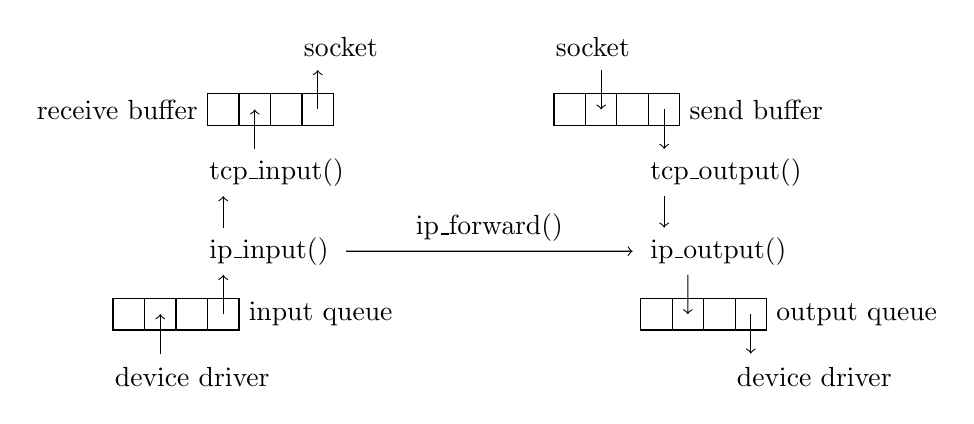
\begin{tikzpicture}
  \draw (0,0)
    node (idd) [right] {device driver} ++(.1,.6)
    rectangle ++(.4,.4) rectangle ++(.4,-.4)
    rectangle ++(.4,.4) rectangle ++(.4,-.4) ++(0,.2)
    node (iq) [right] {input queue} ++(-.5,.8)
    node (ii) [right] {ip\_input()} ++(0,1.0)
    node (ti) [right] {tcp\_input()} ++(.1,.8)
    node (rb) [left] {receive buffer} ++(0,-.2)
    rectangle ++(.4,.4) rectangle ++(.4,-.4)
    rectangle ++(.4,.4) rectangle ++(.4,-.4) ++(-.5,1.0)
    node (iso) [right] {socket} ++(3.2,0)

    node (oso) [right] {socket} ++(.1,-.6)
    rectangle ++(.4,-.4) rectangle ++(.4,.4)
    rectangle ++(.4,-.4) rectangle ++(.4,.4) ++(0,-.2)
    node (sb) [right] {send buffer} ++(-.5,-.8)
    node (to) [right] {tcp\_output()} ++(0,-1.0)
    node (io) [right] {ip\_output()} ++(0,-.6)
    rectangle ++(.4,-.4) rectangle ++(.4,.4)
    rectangle ++(.4,-.4) rectangle ++(.4,.4) ++(0,-.2)
    node (oq) [right] {output queue} ++(-.5,-.8)
    node (odd) [right] {device driver}
    ;
  \path (node cs:name=idd,anchor=west) +(.3+1*.4,.3) coordinate (iddo) {};
  \path (node cs:name=iq,anchor=west) +(-.2-2*.4,0) coordinate (iqi) {};
  \draw[->] (iddo) -- (iqi);
  \path (node cs:name=iq,anchor=west) +(-.2,0) coordinate (iqo) {};
  \path (node cs:name=ii,anchor=west) +(.3,-.3) coordinate (iii) {};
  \draw[->] (iqo) -- (iii);
  \path (node cs:name=ii,anchor=west) +(.3,.3) coordinate (iio) {};
  \path (node cs:name=ti,anchor=west) +(.3,-.3) coordinate (tii) {};
  \draw[->] (iio) -- (tii);
  \path (node cs:name=ti,anchor=west) +(.3+1*.4,.3) coordinate (iti) {};
  \path (node cs:name=rb,anchor=east) +(.2+1*.4,0) coordinate (rbi) {};
  \draw[->] (iti) -- (rbi);
  \path (node cs:name=rb,anchor=east) +(.2+3*.4,0) coordinate (rbo) {};
  \path (node cs:name=iso,anchor=west) +(.3,-.3) coordinate (isoi) {};
  \draw[->] (rbo) -- (isoi);

  \path (node cs:name=oso,anchor=west) +(.3+1*.4,-.3) coordinate (osoo) {};
  \path (node cs:name=sb,anchor=west) +(-.2-2*.4,0) coordinate (sbi) {};
  \draw[->] (osoo) -- (sbi);
  \path (node cs:name=sb,anchor=west) +(-.2,0) coordinate (sbo) {};
  \path (node cs:name=to,anchor=west) +(.3,.3) coordinate (toi) {};
  \draw[->] (sbo) -- (toi);
  \path (node cs:name=to,anchor=west) +(.3,-.3) coordinate (too) {};
  \path (node cs:name=io,anchor=west) +(.3,.3) coordinate (ioi) {};
  \draw[->] (too) -- (ioi);
  \path (node cs:name=io,anchor=west) +(.6,-.3) coordinate (ioo) {};
  \path (node cs:name=oq,anchor=west) +(-.2-2*.4,0) coordinate (oqi) {};
  \draw[->] (ioo) -- (oqi);
  \path (node cs:name=oq,anchor=west) +(-.2,0) coordinate (oqo) {};
  \path (node cs:name=odd,anchor=west) +(.3,.3) coordinate (oddi) {};
  \draw[->] (oqo) -- (oddi);

  \path (node cs:name=ii,anchor=east) +(.1,0) coordinate (ifo) {};
  \path (node cs:name=io,anchor=west) +(-.1,0) coordinate (ifi) {};
  \draw[->] (ifo) -- (ifi) node [midway,above] {ip\_forward()};
\end{tikzpicture}
\end{frame}

\subsection{Towards Parallel Processing}
\begin{frame}{Towards Parallel Processing}
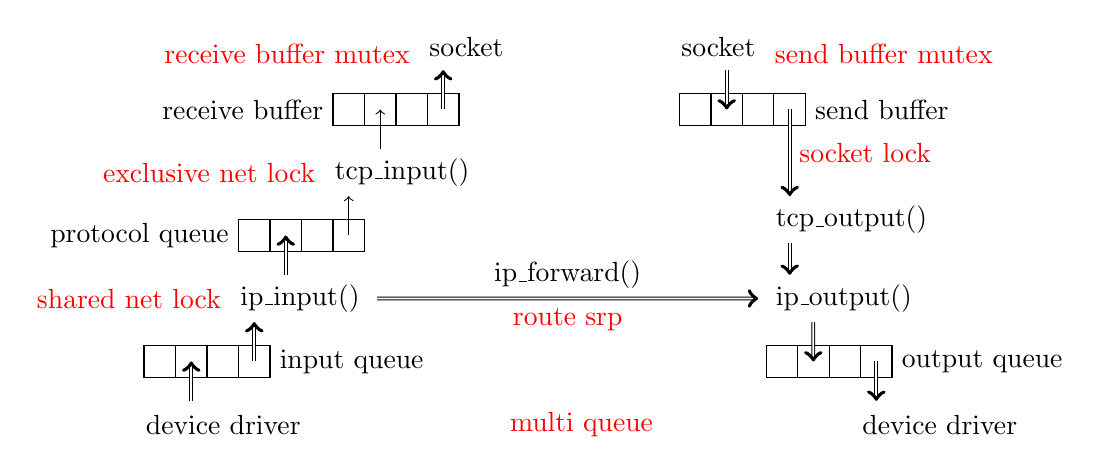
\begin{tikzpicture}
  \draw (0,0)
    node (idd) [right] {device driver} ++(.1,.6)
    rectangle ++(.4,.4) rectangle ++(.4,-.4)
    rectangle ++(.4,.4) rectangle ++(.4,-.4) ++(0,.2)
    node (iq) [right] {input queue} ++(-.5,.8)
    node (ii) [right] {ip\_input()} ++(.1,.8)
    node (pq) [left] {protocol queue} ++(0,-.2)
    rectangle ++(.4,.4) rectangle ++(.4,-.4)
    rectangle ++(.4,.4) rectangle ++(.4,-.4) ++(-.5,1.0)
    node (ti) [right] {tcp\_input()} ++(.1,.8)
    node (rb) [left] {receive buffer} ++(0,-.2)
    rectangle ++(.4,.4) rectangle ++(.4,-.4)
    rectangle ++(.4,.4) rectangle ++(.4,-.4) ++(-.5,1.0)
    node (iso) [right] {socket} ++(3.2,0)

    node (oso) [right] {socket} ++(.1,-.6)
    rectangle ++(.4,-.4) rectangle ++(.4,.4)
    rectangle ++(.4,-.4) rectangle ++(.4,.4) ++(0,-.2)
    node (sb) [right] {send buffer} ++(-.5,-1.4)
    node (to) [right] {tcp\_output()} ++(0,-1.0)
    node (io) [right] {ip\_output()} ++(0,-.6)
    rectangle ++(.4,-.4) rectangle ++(.4,.4)
    rectangle ++(.4,-.4) rectangle ++(.4,.4) ++(0,-.2)
    node (oq) [right] {output queue} ++(-.5,-.8)
    node (odd) [right] {device driver}
    ;
  \path (node cs:name=idd,anchor=west) +(.3+1*.4,.3) coordinate (iddo) {};
  \path (node cs:name=iq,anchor=west) +(-.2-2*.4,0) coordinate (iqi) {};
  \draw[->,double] (iddo) -- (iqi);
  \path (node cs:name=iq,anchor=west) +(-.2,0) coordinate (iqo) {};
  \path (node cs:name=ii,anchor=west) +(.3,-.3) coordinate (iii) {};
  \draw[->,double] (iqo) -- (iii);
  \path (node cs:name=ii,anchor=west) +(.3+1*.4,.3) coordinate (iio) {};
  \path (node cs:name=pq,anchor=east) +(.2+1*.4,0) coordinate (pqi) {};
  \draw[->,double] (iio) -- (pqi);
  \path (node cs:name=pq,anchor=east) +(.2+3*.4,0) coordinate (pqo) {};
  \path (node cs:name=ti,anchor=west) +(.3,-.3) coordinate (tii) {};
  \draw[->] (pqo) -- (tii);
  \path (node cs:name=ti,anchor=west) +(.3+1*.4,.3) coordinate (iti) {};
  \path (node cs:name=rb,anchor=east) +(.2+1*.4,0) coordinate (rbi) {};
  \draw[->] (iti) -- (rbi);
  \path (node cs:name=rb,anchor=east) +(.2+3*.4,0) coordinate (rbo) {};
  \path (node cs:name=iso,anchor=west) +(.3,-.3) coordinate (isoi) {};
  \draw[->,double] (rbo) -- (isoi);

  \path (node cs:name=oso,anchor=west) +(.3+1*.4,-.3) coordinate (osoo) {};
  \path (node cs:name=sb,anchor=west) +(-.2-2*.4,0) coordinate (sbi) {};
  \draw[->,double] (osoo) -- (sbi);
  \path (node cs:name=sb,anchor=west) +(-.2,0) coordinate (sbo) {};
  \path (node cs:name=to,anchor=west) +(.3,.3) coordinate (toi) {};
  \draw[->,double] (sbo) -- (toi);
  \path (node cs:name=to,anchor=west) +(.3,-.3) coordinate (too) {};
  \path (node cs:name=io,anchor=west) +(.3,.3) coordinate (ioi) {};
  \draw[->,double] (too) -- (ioi);
  \path (node cs:name=io,anchor=west) +(.6,-.3) coordinate (ioo) {};
  \path (node cs:name=oq,anchor=west) +(-.2-2*.4,0) coordinate (oqi) {};
  \draw[->,double] (ioo) -- (oqi);
  \path (node cs:name=oq,anchor=west) +(-.2,0) coordinate (oqo) {};
  \path (node cs:name=odd,anchor=west) +(.3,.3) coordinate (oddi) {};
  \draw[->,double] (oqo) -- (oddi);

  \path (node cs:name=ii,anchor=east) +(.1,0) coordinate (ifo) {};
  \path (node cs:name=io,anchor=west) +(-.1,0) coordinate (ifi) {};
  \draw[->,double] (ifo) -- (ifi) node [midway,above] {ip\_forward()};

  \draw[red] (node cs:name=iso,anchor=west) +(0,-.1)
    node [left] {receive buffer mutex};
  \draw[red] (node cs:name=oso,anchor=east) +(0,-.1)
    node [right] {send buffer mutex};
  \draw[red] (node cs:name=ti,anchor=west) node [left] {exclusive net lock};
  \path (sbo) -- (toi) node [red,midway,right] {socket lock};
  \draw[red] (node cs:name=ii,anchor=west) node [left] {shared net lock};
  \path (ifo) -- (ifi) node [red,midway,below] {route srp};
  \path (idd) -- (odd) node [red,midway] {multi queue};
\end{tikzpicture}
\end{frame}

\subsection{Parallel TCP Input}
\begin{frame}{Parallel TCP Input}
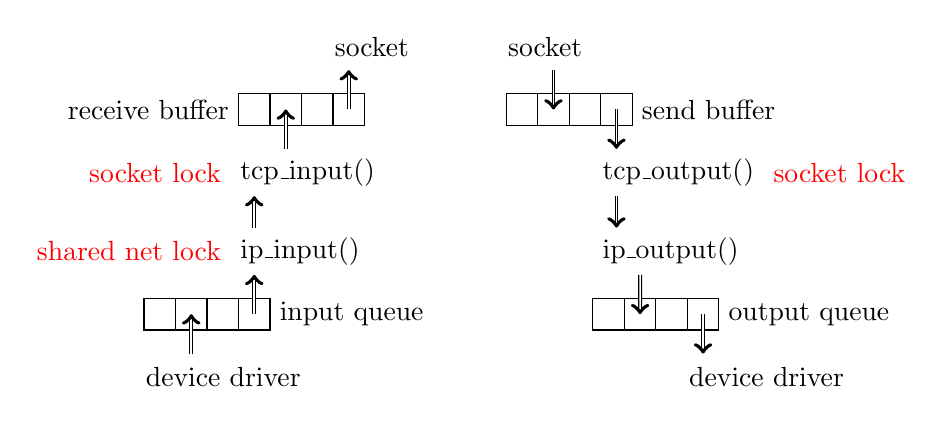
\begin{tikzpicture}
  \draw (0,0)
    node (idd) [right] {device driver} ++(.1,.6)
    rectangle ++(.4,.4) rectangle ++(.4,-.4)
    rectangle ++(.4,.4) rectangle ++(.4,-.4) ++(0,.2)
    node (iq) [right] {input queue} ++(-.5,.8)
    node (ii) [right] {ip\_input()} ++(0,1.0)
    node (ti) [right] {tcp\_input()} ++(.1,.8)
    node (rb) [left] {receive buffer} ++(0,-.2)
    rectangle ++(.4,.4) rectangle ++(.4,-.4)
    rectangle ++(.4,.4) rectangle ++(.4,-.4) ++(-.5,1.0)
    node (iso) [right] {socket} ++(2.2,0)

    node (oso) [right] {socket} ++(.1,-.6)
    rectangle ++(.4,-.4) rectangle ++(.4,.4)
    rectangle ++(.4,-.4) rectangle ++(.4,.4) ++(0,-.2)
    node (sb) [right] {send buffer} ++(-.5,-.8)
    node (to) [right] {tcp\_output()} ++(0,-1.0)
    node (io) [right] {ip\_output()} ++(0,-.6)
    rectangle ++(.4,-.4) rectangle ++(.4,.4)
    rectangle ++(.4,-.4) rectangle ++(.4,.4) ++(0,-.2)
    node (oq) [right] {output queue} ++(-.5,-.8)
    node (odd) [right] {device driver}
    ;
  \path (node cs:name=idd,anchor=west) +(.3+1*.4,.3) coordinate (iddo) {};
  \path (node cs:name=iq,anchor=west) +(-.2-2*.4,0) coordinate (iqi) {};
  \draw[->,double] (iddo) -- (iqi);
  \path (node cs:name=iq,anchor=west) +(-.2,0) coordinate (iqo) {};
  \path (node cs:name=ii,anchor=west) +(.3,-.3) coordinate (iii) {};
  \draw[->,double] (iqo) -- (iii);
  \path (node cs:name=ii,anchor=west) +(.3,.3) coordinate (iio) {};
  \path (node cs:name=ti,anchor=west) +(.3,-.3) coordinate (tii) {};
  \draw[->,double] (iio) -- (tii);
  \path (node cs:name=ti,anchor=west) +(.3+1*.4,.3) coordinate (iti) {};
  \path (node cs:name=rb,anchor=east) +(.2+1*.4,0) coordinate (rbi) {};
  \draw[->,double] (iti) -- (rbi);
  \path (node cs:name=rb,anchor=east) +(.2+3*.4,0) coordinate (rbo) {};
  \path (node cs:name=iso,anchor=west) +(.3,-.3) coordinate (isoi) {};
  \draw[->,double] (rbo) -- (isoi);

  \path (node cs:name=oso,anchor=west) +(.3+1*.4,-.3) coordinate (osoo) {};
  \path (node cs:name=sb,anchor=west) +(-.2-2*.4,0) coordinate (sbi) {};
  \draw[->,double] (osoo) -- (sbi);
  \path (node cs:name=sb,anchor=west) +(-.2,0) coordinate (sbo) {};
  \path (node cs:name=to,anchor=west) +(.3,.3) coordinate (toi) {};
  \draw[->,double] (sbo) -- (toi);
  \path (node cs:name=to,anchor=west) +(.3,-.3) coordinate (too) {};
  \path (node cs:name=io,anchor=west) +(.3,.3) coordinate (ioi) {};
  \draw[->,double] (too) -- (ioi);
  \path (node cs:name=io,anchor=west) +(.6,-.3) coordinate (ioo) {};
  \path (node cs:name=oq,anchor=west) +(-.2-2*.4,0) coordinate (oqi) {};
  \draw[->,double] (ioo) -- (oqi);
  \path (node cs:name=oq,anchor=west) +(-.2,0) coordinate (oqo) {};
  \path (node cs:name=odd,anchor=west) +(.3,.3) coordinate (oddi) {};
  \draw[->,double] (oqo) -- (oddi);

  \path (node cs:name=ii,anchor=east) +(.1,0) coordinate (ifo) {};
  \path (node cs:name=io,anchor=west) +(-.1,0) coordinate (ifi) {};

  \draw[red] (node cs:name=ti,anchor=west) node [left] {socket lock};
  \draw[red] (node cs:name=to,anchor=east) node [right] {socket lock};
  \draw[red] (node cs:name=ii,anchor=west) node [left] {shared net lock};
\end{tikzpicture}
\end{frame}

\section{Performance}

\subsection{Variants for TCP Input}
\begin{frame}{Variants for TCP Input}
\begin{tikzpicture}
  \path (0,0) node [anchor=south west] {
    \begin{adjustbox}{width=\textwidth-0\baselineskip}
      \input{gnuplot/2025-01-26T17-08-00Z-tcp-0,1,2,3.tex}
    \end{adjustbox}
  };
  \path[red,font=\small]
    (3.8,1.5) node [anchor=south] {exclusive} node [anchor=center] {net lock}
    ++(2.4,0) node [anchor=south] {goal}
    ++(2.4,0) node [anchor=south] {cost of} node [anchor=center] {socket lock}
    ++(2.4,0) node [anchor=south] {parallel} node [anchor=center] {TCP input}
  ;
\end{tikzpicture}
\end{frame}

\subsection{Exclusive TCP Receive Single Stream}
\begin{frame}{Exclusive TCP Receive Single Stream}
    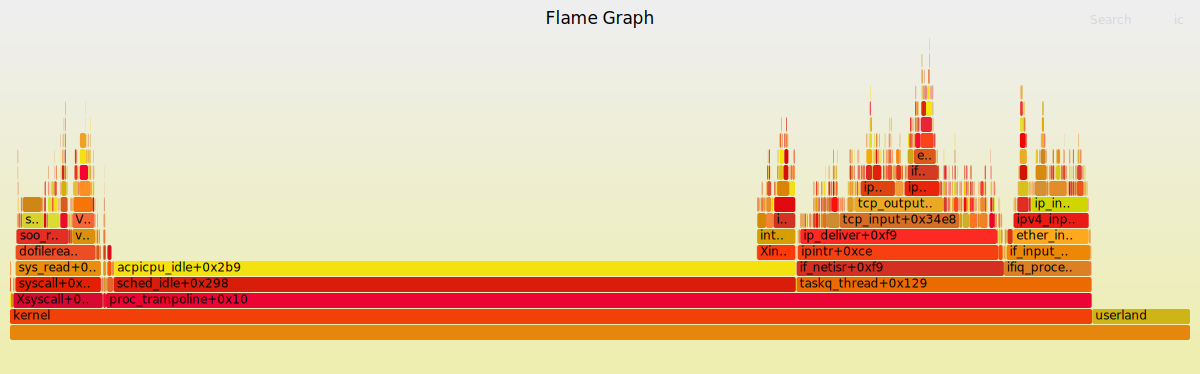
\includegraphics[width=\textwidth]{kstack/sys-tcp-input-solock-rev-single.pdf}
\end{frame}

\subsection{Parallel TCP Receive Single Stream}
\begin{frame}{Parallel TCP Receive Single Stream}
\begin{tikzpicture}
  \path (0,0) node [anchor=south west] {
    \begin{adjustbox}{width=\textwidth-0\baselineskip}
      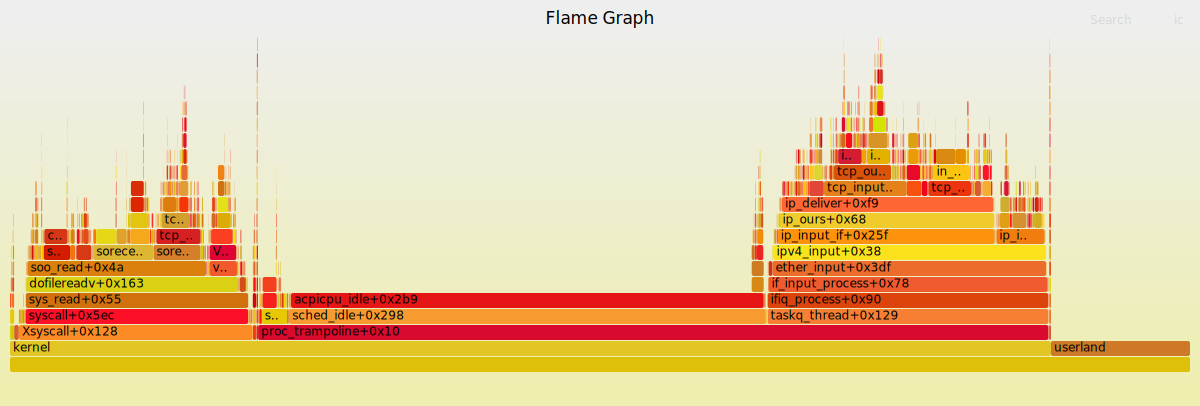
\includegraphics[width=\textwidth]{kstack/sys-tcp-mpinput-rev-single.pdf}
    \end{adjustbox}
  };
  \path[ellipse,black,thick]
    (1.6,2.15) node [draw,minimum width=.8cm,minimum height=.2cm] {}
    (11.25,3.05) node [draw,minimum width=.5cm,minimum height=.2cm] {}
  ;
\end{tikzpicture}
\end{frame}

\subsection{Parallel TCP Input, Socket Lock per Thread}
\begin{frame}{Parallel TCP Input, Socket Lock per Thread}
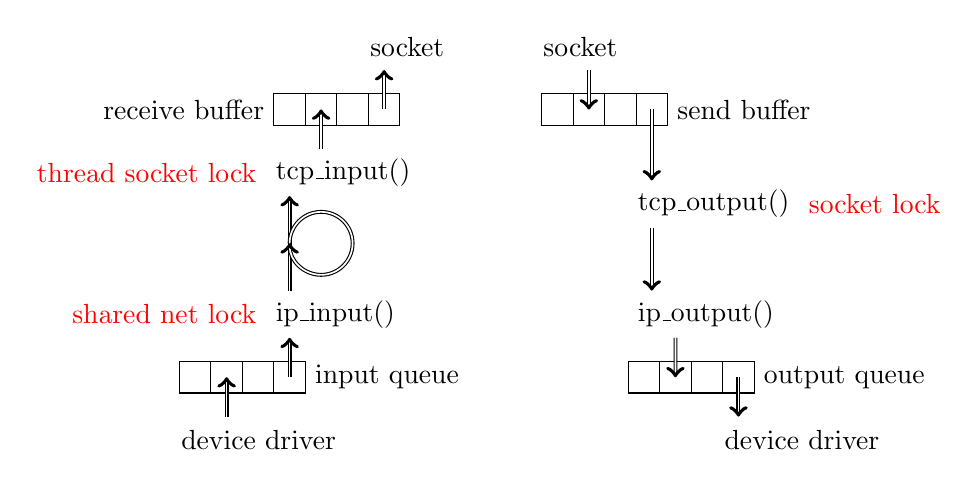
\begin{tikzpicture}
  \draw (0,0)
    node (idd) [right] {device driver} ++(.1,.6)
    rectangle ++(.4,.4) rectangle ++(.4,-.4)
    rectangle ++(.4,.4) rectangle ++(.4,-.4) ++(0,.2)
    node (iq) [right] {input queue} ++(-.5,.8)
    node (ii) [right] {ip\_input()} ++(0,1.8)
    node (ti) [right] {tcp\_input()} ++(.1,.8)
    node (rb) [left] {receive buffer} ++(0,-.2)
    rectangle ++(.4,.4) rectangle ++(.4,-.4)
    rectangle ++(.4,.4) rectangle ++(.4,-.4) ++(-.5,1.0)
    node (iso) [right] {socket} ++(2.2,0)

    node (oso) [right] {socket} ++(.1,-.6)
    rectangle ++(.4,-.4) rectangle ++(.4,.4)
    rectangle ++(.4,-.4) rectangle ++(.4,.4) ++(0,-.2)
    node (sb) [right] {send buffer} ++(-.5,-1.2)
    node (to) [right] {tcp\_output()} ++(0,-1.4)
    node (io) [right] {ip\_output()} ++(0,-.6)
    rectangle ++(.4,-.4) rectangle ++(.4,.4)
    rectangle ++(.4,-.4) rectangle ++(.4,.4) ++(0,-.2)
    node (oq) [right] {output queue} ++(-.5,-.8)
    node (odd) [right] {device driver}
    ;
  \path (node cs:name=idd,anchor=west) +(.3+1*.4,.3) coordinate (iddo) {};
  \path (node cs:name=iq,anchor=west) +(-.2-2*.4,0) coordinate (iqi) {};
  \draw[->,double] (iddo) -- (iqi);
  \path (node cs:name=iq,anchor=west) +(-.2,0) coordinate (iqo) {};
  \path (node cs:name=ii,anchor=west) +(.3,-.3) coordinate (iii) {};
  \draw[->,double] (iqo) -- (iii);
  \path (node cs:name=ii,anchor=west) +(.3,.3) coordinate (iio) {};
  \path (node cs:name=ti,anchor=west) +(.3,-.3) coordinate (tii) {};
  \draw[->,double] (iio) -- (tii) node (tt) [midway] {};
  \draw[->,double] (node cs:name=tt) arc [start angle=360,end angle=0,radius=-.4cm];
  \path (node cs:name=ti,anchor=west) +(.3+1*.4,.3) coordinate (iti) {};
  \path (node cs:name=rb,anchor=east) +(.2+1*.4,0) coordinate (rbi) {};
  \draw[->,double] (iti) -- (rbi);
  \path (node cs:name=rb,anchor=east) +(.2+3*.4,0) coordinate (rbo) {};
  \path (node cs:name=iso,anchor=west) +(.3,-.3) coordinate (isoi) {};
  \draw[->,double] (rbo) -- (isoi);

  \path (node cs:name=oso,anchor=west) +(.3+1*.4,-.3) coordinate (osoo) {};
  \path (node cs:name=sb,anchor=west) +(-.2-2*.4,0) coordinate (sbi) {};
  \draw[->,double] (osoo) -- (sbi);
  \path (node cs:name=sb,anchor=west) +(-.2,0) coordinate (sbo) {};
  \path (node cs:name=to,anchor=west) +(.3,.3) coordinate (toi) {};
  \draw[->,double] (sbo) -- (toi);
  \path (node cs:name=to,anchor=west) +(.3,-.3) coordinate (too) {};
  \path (node cs:name=io,anchor=west) +(.3,.3) coordinate (ioi) {};
  \draw[->,double] (too) -- (ioi);
  \path (node cs:name=io,anchor=west) +(.6,-.3) coordinate (ioo) {};
  \path (node cs:name=oq,anchor=west) +(-.2-2*.4,0) coordinate (oqi) {};
  \draw[->,double] (ioo) -- (oqi);
  \path (node cs:name=oq,anchor=west) +(-.2,0) coordinate (oqo) {};
  \path (node cs:name=odd,anchor=west) +(.3,.3) coordinate (oddi) {};
  \draw[->,double] (oqo) -- (oddi);

  \path (node cs:name=ii,anchor=east) +(.1,0) coordinate (ifo) {};
  \path (node cs:name=io,anchor=west) +(-.1,0) coordinate (ifi) {};

  \draw[red] (node cs:name=ti,anchor=west) node [left] {thread socket lock};
  \draw[red] (node cs:name=to,anchor=east) node [right] {socket lock};
  \draw[red] (node cs:name=ii,anchor=west) node [left] {shared net lock};
\end{tikzpicture}
\end{frame}

\subsection{TCP Receive Parallel Stream, Socket Lock per Thread}
\begin{frame}{TCP Receive Parallel Stream, Socket Lock per Thread}
    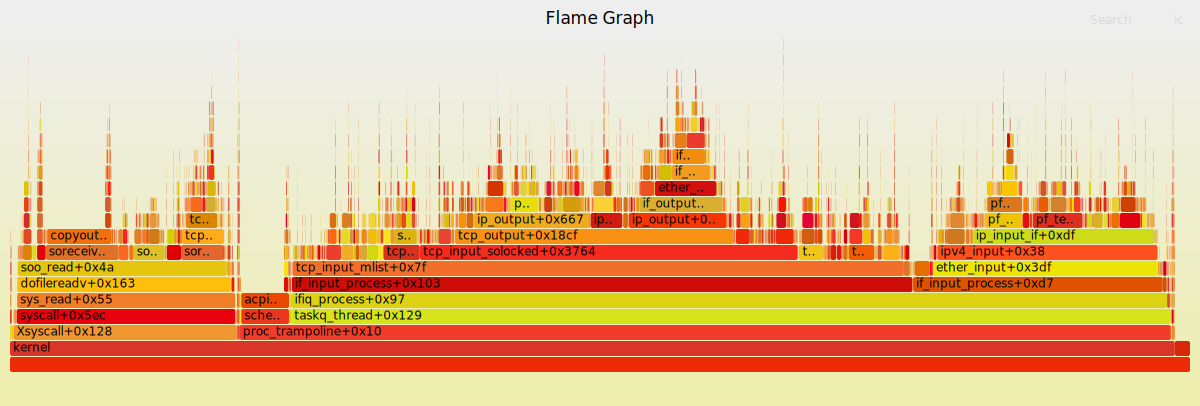
\includegraphics[width=\textwidth]{kstack/sys-tcp-input-parallel-rev-parallel.pdf}
\end{frame}

\subsection{Variants for TCP Input}
\begin{frame}{Variants for TCP Input}
\begin{tikzpicture}
  \path (0,0) node [anchor=south west] {
    \begin{adjustbox}{width=\textwidth-0\baselineskip}
      \input{gnuplot/2025-01-26T17-08-00Z-tcp-0,1,2,3.tex}
    \end{adjustbox}
  };
  \path[red,font=\small]
    (3.8,1.5) node [anchor=south] {exclusive} node [anchor=center] {net lock}
    ++(2.4,0) node [anchor=south] {per thread} node [anchor=center] {socket lock}
    ++(2.4,0) node [anchor=south] {cost of} node [anchor=center] {socket lock}
    ++(2.4,0) node [anchor=south] {parallel} node [anchor=center] {TCP input}
  ;
\end{tikzpicture}
\end{frame}

\end{document}
